\documentclass[acmsmall,screen,review,anonymous]{acmart}

\usepackage{cleveref}
\usepackage{siunitx}
\usepackage{soul}
\usepackage{graphicx}
\usepackage{subcaption}
% \usepackage{enumitem}
\usepackage[inline]{enumitem}
% \usepackage{subfig}

\usepackage[frozencache=false]{minted}
% \definecolor{bg}{rgb}{0.95,0.95,0.95}
\usemintedstyle{colorful}
\setminted[python]{breaklines}
\setminted[python]{xleftmargin=\parindent}
\setminted[python]{bgcolor=bg}


\settopmatter{printfolios=true}
\overfullrule=1mm
%\let\showappendix\relax
\newcommand{\ifappendix}[2]{\ifdef{\showappendix}{#1}{#2}}

\newcommand{\code}[1]{\texttt{#1}}
\newcommand{\mypy}{mypy}
\newcommand{\pytype}{\code{PyType}}
\newcommand{\Any}{\code{Any}}
\newcommand{\JSPP}{\code{JS++}}
\newcommand{\pct}[1]{\SI{#1}{\percent}}


\begin{document}

\title{Dynamic Type in the Wild... FILL}

\author{Dibri Nsofor}
\orcid{0009-0003-7599-2657}
\affiliation{
  \department{Kahlert School of Computing}
  \institution{University of Utah}
  \city{Salt Lake City}
  \state{Utah}
  \postcode{84112}
  \country{USA}
}
\email{dibrinsofor@gmail.com}

% \renewcommand{\shortauthors}{}

\begin{abstract}
  % users far reaching, how do we offer better typing support
  This paper reports a 12 week study reporting suggestions and refinement to improve Luau type adoption
\end{abstract}

\maketitle

%% -----------------------------------------------------------------------------

\section{Introduction}
\label{s:intro}
\label{s:background}
Typing serves two primary purposes: as a documentation tool and to 
safeguard code from type-related runtime errors (or logical inconsistencies). 
Language designers have begun retrofitting type systems to untyped languages as some middle ground between the expressivity 
of these languages that make for good prototyping tools and 
the benefits that types offer, with the most common approach to this being 
erasure typing. Erasure types allow developers to gradually add 
type annotations to code that can be checked statically at compile time without 
offering type-based performance optimizations. Unannotated 
positions receive a dynamic type, a top type that is a superset of 
all existing types in the type system, which acts as a wildcard for
when typing becomes restrictive. 

Roblox's Luau \cite{luau_lang} adopts such a type system which allows developers 
to fine-tune type-checking using hot comments to select one 
of three available typing modes: \code{--!nocheck}, \code{--!nonstrict}, 
\code{--!strict}. These configuration settings will
determine what type of errors are exposed to users. \code{--!nocheck}
suppresses all type-related errors but still provides auto-complete suggestions, 
\code{--!nonstrict} will only raise errors 
for compositions that are guaranteed to fail and \code{--!strict} is complete, 
in that it will raise all types of errors.

% how do I fit in the two solvers?

Roblox caters to a wide variety of users, from fledgling 
developers to expert experience creators. Its aim with Luau is to address developer pain 
points when writing scripts for experiences by providing tools that make 
it easier to write, maintain, and interact with Roblox APIs. To identify and address 
possible user pain points, we run two parallel studies: We instrument telemetry 
to study how developers use the dynamic type (any) towards the goal of filling 
any gaps in the type system and experiment with typing existing Roblox experiences 
to improve the typing experience for creators in Studio and probe patterns discovered 
by the data.

This paper presents a progress report of our journey towards improving the overall 
typing experience in Roblox Studio. In the following sections we explore:
 • The design of our telemetry to study the dynamic type (section 3)
 • Early-stage findings regarding the use of the Any type
 • Suggestions regarding the typing experience in Roblox Studio

% \section{Context: State of Luau}
% \label{s:mypy}

% Luau is in the process of transitioning its type inference and type checking engines,
% from 
% FILL odd transition period between the old and new solver.
% FILL how does luau type checker work.

\section{Telemetry Design}
\label{s:approach:1}
We instrumented telemetry for Roblox Studio (Roblox's video game engine) and \code{roblox-cli} 
(Roblox's internal command line utility for the game engine) to track usage of the any type in 
Luau scripts. The telemetry runs after typechecking and walks the AST 
looking for expressions in the code that map to types generated by the solver that 
contain the any type and sends this data to an elastic search data store which we query and 
parse to support our manual analysis. For each instance where we find the any type, we 
collect information about what solver is used (since Luau is in the middle of transitioning 
to a new solver which attempts bidirectional typechecking), the typing mode, source code snippets that 
contains the annotation and the type inferred by the solver.

The telemetry is on by default, precisely because it is carefully designed to be as minimal as 
possible. FILL profile results. It is, however, also wrapped in its own flag allowing users to opt-out of the study, 
if they desire. Following guidelines from the previous study tracking errors \cite{gtnffvf-jfp-2019}, we make 
extra effort to ensure the data collected cannot be tied back to specific experiences or users. 
As language designers, we can gather a lot of data during a short time to further improve the 
language and then disable the telemetry, repeating this process as the language grows. So far, we 
have collected FILL records of interest over 4 weeks and have begun a manual 
analysis studying why the \code{Any} type shows up and how we can better support users 
on the platform.

\begin{figure}[t]
  \centering
  {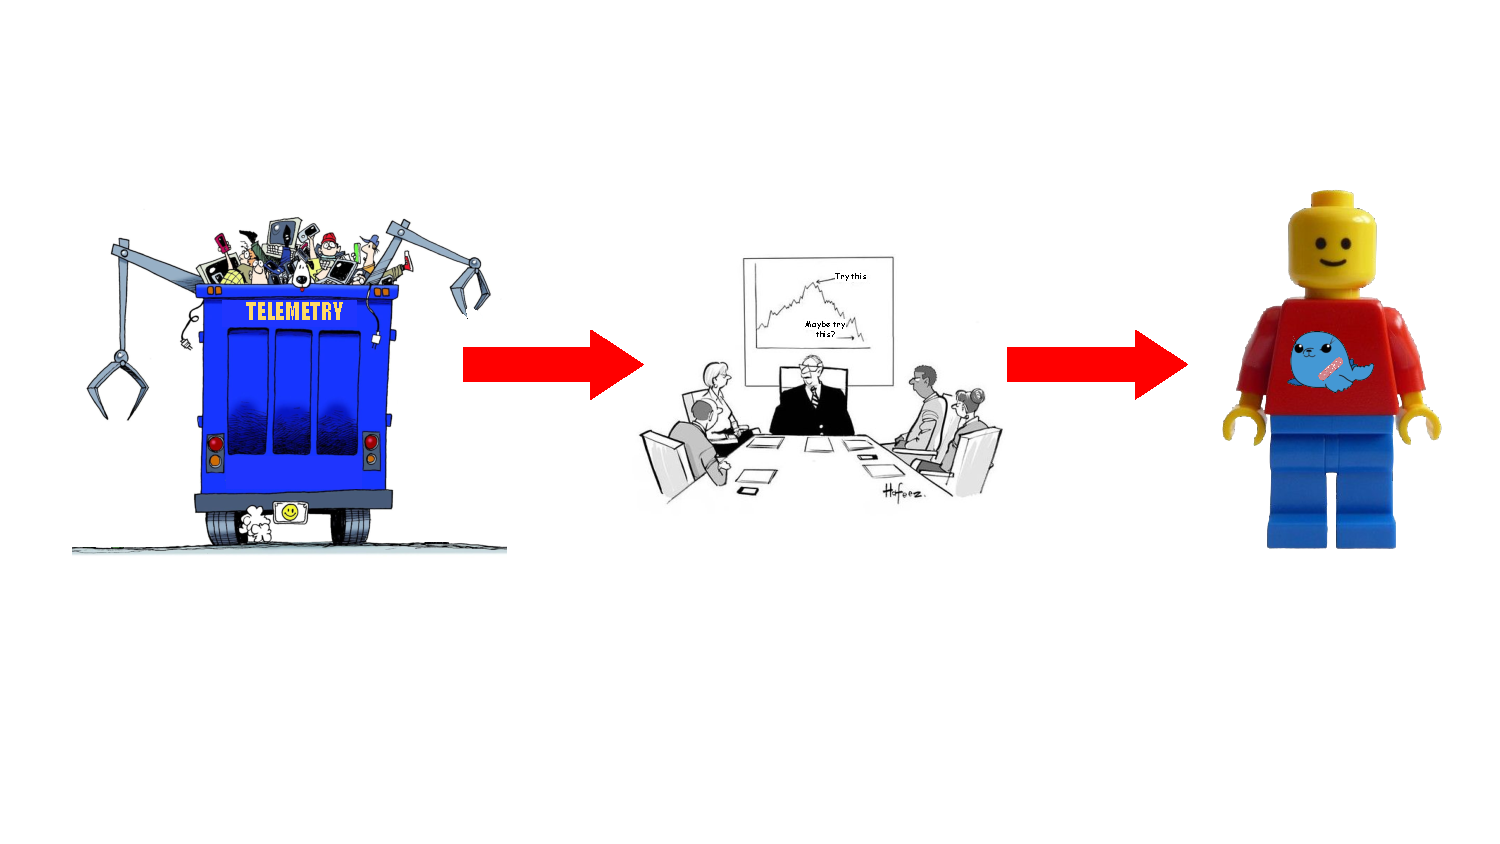
\includegraphics[width=0.66\columnwidth,trim={140 120 140 100}]{src/images/telemetry.pdf}}
  \caption{Telemetry study overview}
  \label{f:approach}
\end{figure}


Currently, we are in the midst of an initial stage of the project in which we study 
instances of the dynamic type by hand. Particularly seeking out areas where 
we could either implement autocomplete suggestions to replace \Any{}s in code or 
suggest more precise types and operators to better support the language's wide 
spectrum of users. More details about the telemetry's implementation can be
seen through the Pull Request \cite{ats_pr}.

FILL running place files. that's most of the data we have.

\subsection{Studying the data}
\label{s:approach:2}
We collect the telemtry data from Kibana as \code{.csv} files and have a script \cite{luau_analysis_script} that parses the data,
separates it by category, such that one file has a JSON representation of all the anys that show up as function 
arguments, and successive files for function applications, type casts, variable declarations and 
function returns. We further examine, line by line, each of the instances collected to identify 
any repeat patterns that hint at some typing pain point for users. We have been able to identify three
of such interesting patterns:

\subsubsection{Anys to Hide unnecessary Details}
\label{s:approach:3}
When precise type details are irrelevant to the current code, 
Roblox creators tend to use the \Any{} type to circumvent having 
to add additional details. They want to 
be sure an argument is a function or a table but do not care about 
declaring parameters (like \code{{[string]: number}}). Most often creators 
have to mangle unpredictable data between users and the DM so this pattern is 
tells a clear story, they often want outer shape checks. \\
\begin{minted}{lua}
-- 1
export type AnyFunction = ()->( any)
-- 2
type Callback = (...any?)->( ...any?)
-- 3
export type Table = {[any]: any}
\end{minted}
This example code highlights three distinct instances caught by the telemetry
where users carefully adopt the \Any{} type to enforce top level checks. 
Now a function parameter that expects the `AnyFunction' type is forced to check that
a `number' is not supplied but will be permissive to any function type, including
\code{(unknown) -> boolean} and \code{(Table) -> Array<any>}.
Luau supports refinement typing, which allows you to make additional claims about 
data like this, and bidirectional typing, with one of the rules being it will try to 
infer the type for parameters like this after an argument is supplied to the function
to improve the typing experience. One obvious suggestion here would be to remind users
of the benefits of unknowns over any and leveraging type refinements. Additionally,
since users already use this, Luau could ship a type alias that points to the 
supertype of functions (\code{(...unknown) -> ()}) and tables \code{[unknown]: unknown} 
for this intent.
% can bounded generics solve this?
% type Callback<T> = T :: (...unknown) -> ()


% it would be interesting if checking could conflict with inference here in nonstrict mode

\indent{Anys for Circular Import Dependencies}
\label{s:approach:4}
Roblox creators often work across a number of modules and shared scripts which may 
depend on one another, by introducing Luau, creators have now begun to add types to 
the list of exports. If code is not structured properly, users can run into errors 
arising from cyclic dependencies and to suppress such errors, creators have begun type 
casting entire \code{require} expressions to the \Any{} type. We conjecture, that some 
of these dependencies may arise from type defintions. \\
\begin{minted}{lua}
-- module A
local A = require(script.B)

-- module B
local B = require(script.A) :: any -- cyclic dependency fixed with any
\end{minted} 
To remedy this, we suggest maintaining type modules for each project with shared type 
definitions. An alternative suggestion would be to raise this as a warning and not an 
error, if types are the root cause of the dependency issue since types do not affect 
runtime behaviour.

\indent{Anys and the Data Model}
\label{s:approach:5}
The most seemingly trivial cases where anys show up are in compositions that aim to 
interact with parts of the Data Model or Roblox APIs. We imagine users try to use 
Instance names as types and either resort to \Any{} when that does not work or raises
type errors they do not quite clearly understand. Our suggestion here is to expose a 
type module of the DM to users who can lend a hand to improving those types.

\section{Corpus Study}
\label{s:place}

Our parallel study involved adding types to untyped Roblox experiences.
To test improvements made to the solver do not break backwards compatibility, 
the team regularly runs new changes against a corpus of existing experiences 
generated from the cloud. We leverage this corpus for this part of our study.
We select a random sample of three experiences (or Place Files) 
with at least 20 Luau scripts ranging from 3 lines to 100+ lines 
and set out to find any areas where we would either be forced to adopt 
the \Any{} type or notice a lapse in Roblox Studio that could impede the 
creator's experience on the platform -- areas that deserve some tweaks 
to improve the typing experience and thus, Luau's type adoption. In this case, 
we identify two major opportunities for growth:

% quick one liner to understand the data model
% think JS dom but for objects in a 3d world
% we have let the team know and they do think it is something worth exploring
% alternative here would be to be able 
\indent{Interacting with the Data Model}
\label{s:place:1}
Roblox's engine exposes concrete (Data) types for objects defined in the Data Model or 
the Roblox APIs. These types tend to have nested hierarchies including other concrete 
types, which make it difficult to tell what properties and methods may exist for different 
\code{Instances}. For new creators, reasoning about these types may be daunting. We 
spent a long time combing through the documentation to fix issues that arose from 
misuse of these Data Types, particularly when the top concrete type enters the flow of 
the program. As a remedy, we suggest on hover IDE support on magic functions and 
\code{Instance} declarations containing minimal information about said \code{Instance} 
and goto links that jump to relevant parts of the data type documentation. This idea 
has been passed along to the relevant team who thinks this would be a great feature 
to include.  We additionally urge creators to be intentional about the use of the 
top type \code{Instance} FILL width subtyping. FILL . We posit this can improve developer productivity and 
reduce the likelihood of Data Model related errors.

\indent{Code Assist Does not work}
\label{s:place:2}
The engine comes equipped with an AI feature called code assist, which aims 
to be a code completion tool to assist users as they write scripts. In theory, 
this should be an amazing feature, however, one of the researchers
found it to be too obtrusive and in many cases, blatantly wrong with suggesting type information.
One of the many perils of gradual typing is that the types cannot often be taken at 
face value and thus should not be used for any training whatsoever. The researcher 
noticed that on clearing type information like \Any{} and \code{unknown}, code assist
would aggressively still infer that and would take a considerable amount of time to fill 
in these suggestions which broke typing flow. To improve this, we suggest only training the model 
with type information in \code{--!strict} mode and wholly generating the suggestions before it is 
presented to users as opposed to forcing the user watch each token be generated.

\subsection{Additional Notes}
FILL.

\subsubsection{Blocked types}
\label{s:add}
% Intro this paragraph. what is the goal with this paragraph?
The new Luau solver, adopts the idea of bidirectional typing or deferred constraint resolution 
which involves inferring types and propagating expected types. When the 
type checker is yet to resolve a type, it adopts a placeholder which it calls a "blocked type". 
Ideally these blocked types should eventually resolve as constraint analysis proceeds, however, 
with self-referential free types or types with deep cyclic structures, these blocked types can often 
go unresolved and show up in on hover messages that creators see in Roblox Studio. This unintentional 
behaviour shows up in many of the telemetry instances we collect.

\subsubsection{Shared Self Types}
\label{s:add:1}
Probing many of these blocked types, reveals a lapse in the type system that the Luau language designers 
are already aware of. When a method is defined, Luau generates a free type to refer to the object instance (self).
That is for a table with $n$ method properties, each self type will refer to a distinct free type. This sometimes? 
makes it difficult for the solver to normalize these types to the same canonical form. An ideal solution
would be to have a generic bound to the table in question and maintain that across all methods. The languages 
design is driven through Request for Comments (RFCs) and a design for shared types has been agreed upon and 
will be implemented in the future.
FILL Example that generates blocked type.

\subsubsection{Equality Saturation and Blocked Types}
\label{s:add:2}
% normalizer, solver, constraint generation. maybe you need to explain the flow of the typechecker somewhere
Equality Saturation promises an optimization technique that non-destructively applies rewrite rules 
to an expression represented in an e-graph until saturation, and a canonical form is reached. This
approach seems extremely exciting to the language designers to replace the current normalization technique
for the type checker. Here, we explore a minimal example that generates a blocked type and explore,
step by step whether equality saturation may be a feasible solution to this problem. 
FILL Example.

\subsection{Future Work}
Our work previews a large-scale data driven approach to discover how
the dynamic type is used in Luau scripts. Our next step is to leave 
the telemetry up to collect more data and continue to test our hypotheses.
Our additional short term goals include, leveraging the data to create educational content and 
improving auto complete suggestions for scripting in Roblox Studio. 
To fill knowledge gaps Roblox creators may have about the type system, we 
have begun working on a open sourced?? typing guide that we plan to 
incrementally grow as more patterns emerge. In addition to this, we still 
seek out poor typing patterns where \Any{}s can be replaced with 
precise types to better improve auto-complete suggestions.

% % go into detail about how each of these would help,
% % present the problem and then a possible path for a fix

% - shared self
% % mypy introduces shared self here -> https://github.com/python/mypy/pull/14041/files

% - go to defintions for datamodel instances
% % shouldnt stop here, i should be able tojump to defintions in m

% - typing guide for new users (discord is great but people should be able to lookup new features)

% - something to addr this: values only optional prior to assignment
% % big research problem with nil, maybe worth exploring

% - non strict mode, some add settings
% % see mypy configs

% - 
% %  It's our programming model with the Roblox's API and data model that has a bit of learning curve

% \subsection{Discussions}
% \label{s:approach:1}
% FILL Reiter the suggestions.
% FILL. 
% - enforcing static types in the presence of untyped code open a complex design space. 
%   - better typing experience for users in non strict mode
%   - make them aware of the risks or some unobtrusive ways to flag contradictions
%   - delete this mode and allow users toggle type checking for blocks of code
%   - expose checked to developers? allow them to maintain type stubs for third party libraries.
% - improved error reporting, type packs and blame

% How is this helpful to roblox. 
% - improve luau typing experience in Studio
% - fill in gaps in the type system - error reporting, suggest types
% - improve creator facing docs

\bibliographystyle{ACM-Reference-Format}
\bibliography{bib.bib}

\end{document}
\endinput
